\documentclass[border=10pt]{standalone}
\usepackage{tikz}\usepackage{amsmath}\usetikzlibrary{arrows.meta}
\begin{document}
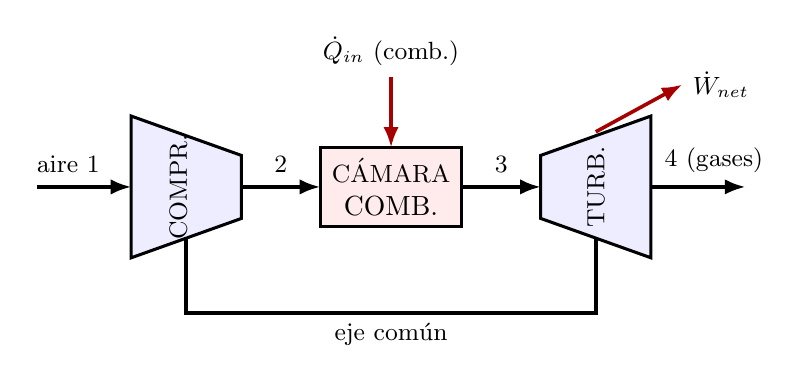
\begin{tikzpicture}[line width=1pt,>={Latex[length=2.6mm]}]
  % compresor (trapezoid que ensancha hacia adentro)
  \fill[blue!7] (0,0.3)--(0,2.1)--(1.4,1.6)--(1.4,0.8)--cycle;
  \draw[line width=1.1pt] (0,0.3)--(0,2.1)--(1.4,1.6)--(1.4,0.8)--cycle;
  \node[rotate=90] at (0.6,1.2){\small COMPR.};
  % camara de combustion
  \fill[red!8] (2.4,0.7) rectangle (4.2,1.7); \draw[line width=1.1pt] (2.4,0.7) rectangle (4.2,1.7);
  \node[align=center] at (3.3,1.2){\small CÁMARA\\COMB.};
  % turbina (ensancha hacia afuera)
  \fill[blue!7] (5.2,0.8)--(5.2,1.6)--(6.6,2.1)--(6.6,0.3)--cycle;
  \draw[line width=1.1pt] (5.2,0.8)--(5.2,1.6)--(6.6,2.1)--(6.6,0.3)--cycle;
  \node[rotate=90] at (5.9,1.2){\small TURB.};
  % conexiones
  \draw[->,line width=1.2pt] (-1.2,1.2)--(0,1.2); \node[above] at (-0.8,1.25){\small aire 1};
  \draw[->,line width=1.2pt] (1.4,1.2)--(2.4,1.2); \node[above] at (1.9,1.25){\small 2};
  \draw[->,line width=1.2pt] (4.2,1.2)--(5.2,1.2); \node[above] at (4.7,1.25){\small 3};
  \draw[->,line width=1.2pt] (6.6,1.2)--(7.8,1.2); \node[above] at (7.4,1.25){\small 4 (gases)};
  % eje comun
  \draw[line width=1.4pt] (0.7,0.55)--(0.7,-0.4)--(5.9,-0.4)--(5.9,0.55);
  \node[below] at (3.3,-0.4){\small eje común};
  % combustible y trabajo
  \draw[->,red!65!black,line width=1.3pt] (3.3,2.6)--(3.3,1.7); \node[above] at (3.3,2.6){\small $\dot Q_{in}$ (comb.)};
  \draw[->,red!65!black,line width=1.3pt] (5.9,1.9)--(7.0,2.5); \node[right] at (7.0,2.5){\small $\dot W_{net}$};
\end{tikzpicture}
\end{document}
